\subsection{Contexte}

Dans cette partie, nous allons voir ce qu'est l'anorexie mentale et ce qui a été réalisé dans le domaine de la sortie de corps en réalité virtuelle. Pour finir, nous verrons les contraintes à respecter pour créer une illusion en sortie de corps en réalité virtuelle pour aider les personne atteintes d'anorexie mentale.
\subsubsection{Anorexie mentale}

L'anorexie mentale est une maladie faisant partie des troubles du comportement alimentaire. Il s'agit une maladie psychiatrique grave qui touche principalement les femmes au moment de l'adolescence suite à une perte de poids et se présente essentiellement sous la forme de trois symptômes :
\begin{itemize}
\item Une restriction alimentaire entraînant une réduction drastique des apports énergétiques malgré les besoins physiologiques.
\item Une peur importante de reprendre du poids.
\item Une mauvaise représentation de son corps.
\end{itemize}

Les personnes touchées par cette maladie surestiment leur poids et leur silhouette, ce qui stoppe ou ralentit le processus de renutrition. Pour déterminer la source de cette mauvaise représentation du corps, Guardia et al. \cite{gu10} ont mis en place une expérience dans laquelle une personne est face à un mur sur lequel est projeté une porte dont la largeur varie. La personne doit alors dire si elle peut passer la porte sans tourner les épaules. Cette expérience a été faite sur des personnes en bonne santé et des personnes atteintes d'anorexie mentale. Ils ont pu observer que les personnes souffrant d'anorexie mentale se tournaient bien avant les autres personnes. Ces résultats tendent à indiquer que le schéma corporel, qui est une représentation sensorimotrice du corps sollicité pour gérer la posture et les actions du corps, serait faussé chez les patients.\\

 Comme le schéma corporel est supposé être basé sur une intégration multisensorielle, l'illusion de la main en caoutchouc ("\emph{Rubber Hand Illusion}") \cite{Bo98} (Voir Figure \ref{fig1}), qui se base sur la création de conflit dans le processus d'intégration multisensorielle, a été réalisée sur des patients souffrants d'anorexie mentale. L'illusion a pour but de faire croire à la personne que la main en caoutchouc fait partie de son corps. Pour cela, une des mains de la personne est cachée et une main en caoutchouc est placée devant elle. Ensuite, la main cachée et la main en caoutchouc sont touchées, par un bâton ou un pinceau par exemple, simultanément ce qui provoque un conflit entre ce qui est vu, la main en caoutchouc touchée par un pinceau, et ce qui est ressenti, la sensation de toucher créée par le pinceau sur la main cachée. Une fois l'illusion créée, on peut ne caresser que la main en caoutchouc. Cette illusion s'est avérée très forte chez les personnes atteintes d'anorexie mentale.\\

Pour aider les patients souffrants d'anorexie mentale, il faut d'abord les aider à corriger la mauvaise représentation qu'ils ont de leurs corps. Pour cela il faut pouvoir modifier la perception qu'ils ont de leur corps. L'illusion de la main en caoutchouc permet de le faire uniquement sur une partie du corps mais elle est très efficace sur eux. Donc la sortie de corps qui repose sur le même principe que cette illusion mais en l'étendant à tout le corps devrait également être efficace sur les personnes atteintes d'anorexie mentale.
\begin{figure}[h]
   	\centerline{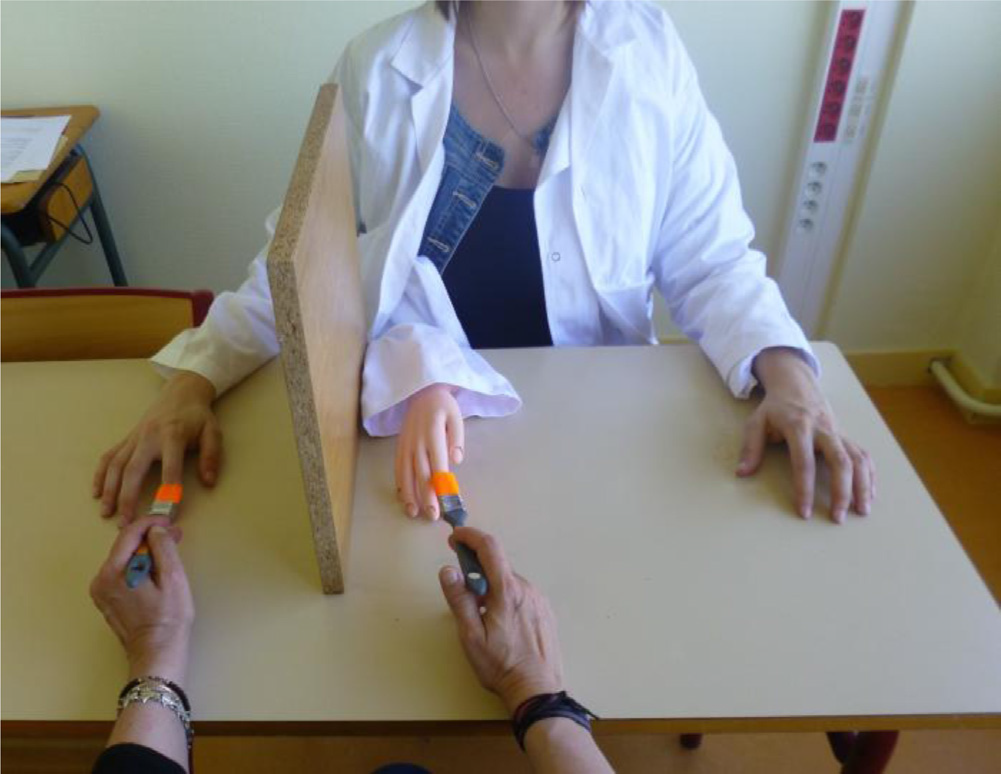
\includegraphics[scale=0.4]{images/biblio/rubberhand}}
   	\caption{\label{fig1} Illusion de la main en caoutchouc \cite{lu14}}
\end{figure}


\subsubsection{Sortie de corps}

La sortie de corps est un phénomène dans lequel une personne a l'impression d'apercevoir le monde d'une position surélevée et de voir son corps à l'extérieur de ses limites physiques, d'avoir la sensation d'être désincarnée \cite{bl10}. Dans cette partie nous allons voir différents travaux réalisés pour reproduire ce phénomène en réalité virtuelle. En réalité virtuelle, l'illusion de sortie de corps cherche à créer une sensation d'appartenance d'un corps ou une partie de corps virtuel contrairement à la vrai sortie de corps qui se définit par une désincarnation.

\paragraph{Sortie de corps en réalité virtuelle}

Olaf Blanke et al. \cite{le07}, se sont appuyés sur l'illusion de la main en caoutchouc pour mettre au point leur expérience (voir Figure \ref{fig2}). Dans cette expérience, le sujet porte un casque de réalité virtuelle et est filmé de dos. Le film est envoyé en temps réel au casque porté par la personne ce qui fait qu'elle voit donc une image de son corps projeté devant elle. Le sujet est alors touché à répétition dans le dos par un bâton. Il voit alors une image virtuelle dans laquelle le dos de son corps est touché par un bâton et en même temps ressent une sensation de toucher dans le dos. L'expérience est réalisée dans deux conditions, une où l'image est synchronisée avec la stimulation tactile et une autre où un délai est ajouté pour créer un décalage entre le moment où la personne est touchée par le bâton et le moment où elle se voit touchée par le bâton dans son casque de réalité virtuelle. Avec la synchronisation, les sujets avaient l'impression que la sensation de toucher venait du fait que le corps virtuel qu’ils percevaient via le casque était touché par un bâton. \'{E}galement, en demandant aux sujets, après qu'ils se soient déplacés, de se remettre à la position où ils étaient, ils avaient tendance à se placer plus près de là où leur corps virtuel était projeté qu'il ne l'était en vrai. Ceci tend à montrer qu'ils se sont identifiés au corps virtuel. Par contre, dans le cas où il n'y avait pas de synchronisation, ces erreurs d'assimilation étaient plus rares.\\

Simuler une attaque sur le faux corps, avec un couteau ou un marteau, peut même augmenter la conductance de la peau ce qui montre une réponse émotionnelle lorsque le corps virtuel est menacé \cite{eh07}. Le même résultat a pu être obtenu en filmant un mannequin de dos touché par un bâton au lieu de filmer directement la personne de dos, même si dans ce cas-là il faut aussi que le sujet soit également touché dans le dos de manière synchronisée par rapport au mannequin \cite{le07}.\\

\begin{figure}[h]
   	\centerline{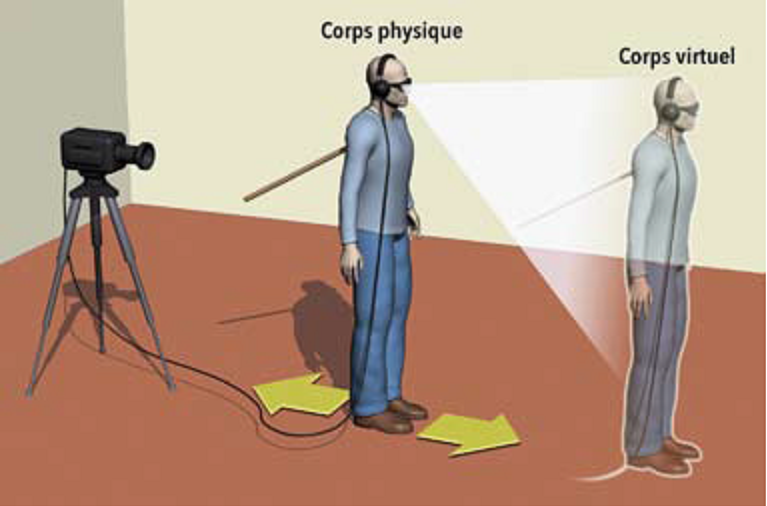
\includegraphics[scale=0.6]{images/biblio/oobRV}}
   	\caption{\label{fig2} Exemple de sortie de corps en Réalité Virtuelle \cite{bl10}}
\end{figure}

L'illusion de la main en caoutchouc a également était réalisée en réalité virtuelle \cite{sl09}, et elle a été réalisée sans utiliser de stimulation tactile mais en bougeant la main virtuelle pour qu'elle reproduise les mouvements de la main de la personne \cite{sl08}(Voir Figure \ref{fig3}). En utilisant un gant de données pour reproduire les mouvements de la main et des doigts de la personne, ils ont pu constater une tendance à identifier la main virtuelle comme étant une partie du corps. La synchronisation entre les mouvements réalisés par le sujet et ceux fait par la main virtuelle est importante pour créer ce sentiment d'appartenance. Cela permet de penser qu'une sortie de corps pourrait être réalisée en reproduisant le mouvement de la personne sur un avatar virtuel.


\begin{figure}[!h]
   	\centerline{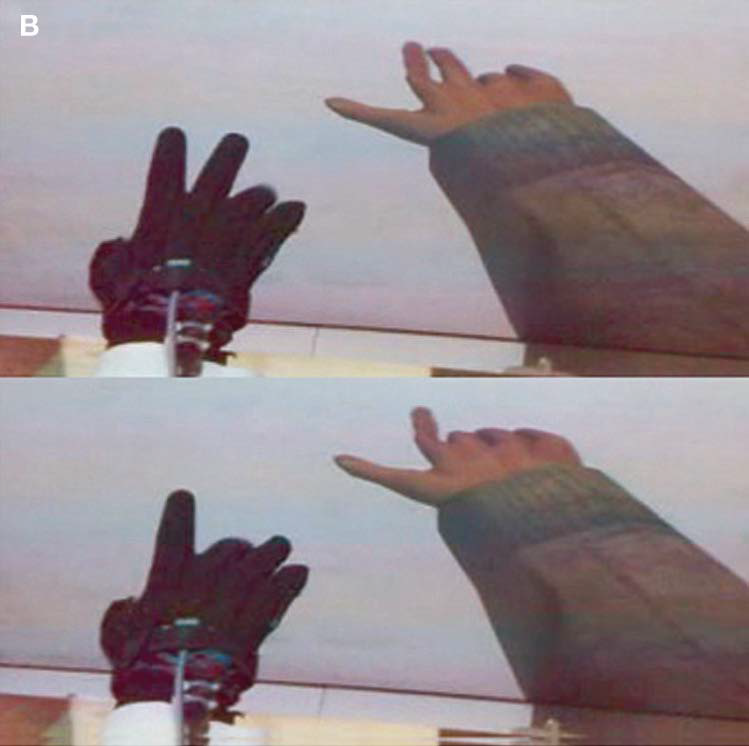
\includegraphics[scale=0.4]{images/biblio/rhiRV}}
   	\caption{\label{fig3} Illusion de la main en caoutchouc en Réalité Virtuelle \cite{sl08}}
\end{figure}


\paragraph{Modification de la perception du corps}

En utilisant la sortie de corps avec des mannequins, Catherine Preston et H. Henrik Ehrsson ont réussi à modifier la satisfaction du corps chez des personnes non atteintes de trouble du comportement alimentaire \cite{pr14}. Pour cela une sortie de corps était réalisée sur les sujets en utilisant un mannequin "maigre" représentant 85\% de la masse corporel du sujet et un mannequin large représentant 115\% de la masse corporel. En utilisant le questionnaire \emph{Body Image States Scale} (BISS) \cite{ca02} qui permet de connaître la satisfaction qu'une personne éprouve par rapport à son corps à l'instant présent, ils ont pu constater une modification dans la satisfaction du corps chez les sujets. Avec la sortie de corps, il a donc été possible chez ces personnes de modifier la satisfaction de leur corps et donc de modifier la perception qu'ils avaient de leur corps. Cependant, l'utilisation de mannequins n'est pas pratique car on ne peut pas changer leurs apparences aisément au niveau de la silhouette. 

\subsubsection{Bilan}
Comme on a pu le voir précédemment, on peut modifier la perception du corps avec la sortie de corps et c'est justement ce que nous souhaitons faire pour aider les personnes atteintes d'anorexie mentale. Seulement l'utilisation de mannequin est limitant, alors qu'avec un modèle 3D d'un corps humain il serait notamment possible de modifier sa silhouette en temps réel. Pour réaliser cela, il faudra également pouvoir capturer les mouvements de la personne et les reproduire avec le modèle 3D. En regardant ce qui a été fait sur la sortie de corps en réalité virtuelle, des sollicitations tactiles sont nécessaires pour créer le phénomène, ce qui signifie qu'il faudra également capturer les mouvements de l'objet (un bâton par exemple) pour réaliser ces actions et reproduire l'objet et ses mouvements dans l'environnement 3D. Cependant, dans le cas de la main en caoutchouc en réalité virtuelle, le fait que la main virtuelle reproduise les mouvements de la vrai main de l'utilisateur permet de se passer des sollicitations tactiles ce qui pourrait aussi être le cas de la sortie de corps. Enfin le dernier point important est la synchronisation, il ne faut pas qu'il y ait de décalage entre ce qui est vu et, soit la sensation de toucher, soit le mouvement effectué, pour créer le phénomène de sortie de corps.

\subsection{Avatar et environnement 3D}
Dans cette section, nous allons voir l'effet que peut avoir un avatar en fonction de son réalisme ainsi que l'impact que peut avoir un environnement virtuel sur notre perception. 
\subsubsection{Apparence de l'avatar}
En utilisant un avatar virtuel, on peut voir apparaitre un effet appelé la \emph{Uncanny Valley} \cite{mo12}. Cet effet représente initialement le fait que dans le domaine de la robotique, plus un robot ressemble à un humain, plus ces défauts gêneront l'utilisateur qui interagit avec lui. Cet effet existe aussi avec les avatar virtuel \cite{mc12} et est accentué lorsque l'avatar réalise des mouvements. Dans cette étude, on peut constater qu'un avatar très réaliste semble familier à l'utilisateur mais qu'il s'agit de l'avatar moyennement réaliste qui semble le moins familier. L'étude regarde aussi l'effet que peut avoir l'apparition d'artefact dans l'animation de l'avatar. Les problèmes d'animations ont moins d'impact lorsque l'avatar n'est pas réaliste et il s'agit de l'avatar moyennement réaliste qui est le plus déplaisant en cas de mauvaise animations. L'interaction avec un avatar ayant une apparence humaine mais pas suffisamment réaliste peut repousser l'utilisateur.
\subsubsection{Perception dans un environnement virtuel}
Pour voir l'impact de la qualité graphique d'un environnement 3D sur la présence ressenti par l'utilisateur, Slater et al. \cite{sla09} on mit des sujets devant un gouffre virtuel, et on analysé la sensation de présence dans l'environnement 3D via questionnaire et les valeurs de conductances de la peau. Suivant les sujets, l'environnement avait des ombres et des réflections dynamiques ou aucunes des deux. Les résultats montre que la présence des ombres et des réflections augmentent ce sentiment de présence.
\subsubsection{Bilan}
Le réalisme de l'apparence de l'avatar peut avoir un impact sur la capacité de l'utilisateur de se lier à lui. Cependant dans le cas d'une sortie de corps où l'utilisateur voit son corps virtuel de dos, rend le visage de l'avatar non visible et ainsi il ne voit pas que l'expression faciale ne corresponde pas à la sienne. Ceci devrait réduire le risque de produire l'effet \emph{Uncanny Valley}. Des critères graphiques comme la présence d'ombre dynamique pour l'avatar pourraient augmenter la présence de l'utilisateur et aider à la création de l'effet de sortie de corps.